% Chapter Template

\chapter{Results} % Main chapter title

\label{Chapter6} % Change X to a consecutive number; for referencing this chapter elsewhere, use \ref{ChapterX}

\lhead{Chapter 6. \emph{Results}} % Change X to a consecutive number; this is for the header on each page - perhaps a shortened title




\section{Results}

We trained our model on all available Mushaf recitations, reserving Mushaf 26.1 and 19.0 exclusively for testing. The evaluation results are summarized in Table \ref{tab:results}. The achieved Average Phoneme Error Rate (PER) of 0.16\% strongly supports our hypothesis that the Quran Phonetic Script is learnable using modern speech processing techniques.

We further tested the model on actual samples containing errors in \arb{مد}, \arb{غنة}, \arb{قلقلة}, and \arb{تفخيم}. Despite being trained only on error-free expert recitations, the model successfully detected these common pronunciation mistakes. While these preliminary results are promising, a more comprehensive evaluation on dedicated error-annotated datasets—such as \cite{khan2021tarteel}—is planned for future work.

We observe that the PER is well-balanced across nearly all phonetic and attribute levels, with the exception of the phoneme level itself. This is expected, as the phoneme level has a significantly larger vocabulary (44 symbols, including padding), increasing its complexity relative to the attribute levels.


\begin{table}[htbp]
\centering
\caption{Test results on Mushaf 26.1 and 19.0. The Average Phoneme Error Rate (PER) is \textbf{0.16\%}, confirming the learnability of the Quran Phonetic Script. The phoneme-level PER is higher (0.54\%) due to its larger vocabulary.}
\label{tab:results}\\
\vspace{3pt}
\label{tab:results}
\begin{tabular}{lc}
\hline
\textbf{Metric} & \textbf{Value} \\
\hline
loss & 0.01162 \\
per\_phonemes & 0.00543 \\
per\_hams\_or\_jahr & 0.00117 \\
per\_shidda\_or\_rakhawa & 0.00172 \\
per\_tafkheem\_or\_taqeeq & 0.00167 \\
per\_itbaq & 0.00092 \\
per\_safeer & 0.00132 \\
per\_qalqla & 0.00085 \\
per\_tikraar & 0.0009 \\
per\_tafashie & 0.0016 \\
per\_istitala & 0.0008 \\
per\_ghonna & 0.0013 \\
average\_per & \textbf{0.0016} \\
\hline
\end{tabular}
\end{table}


To evaluate real-world performance, we developed a demonstration application using Gradio\footnote{https://www.gradio.app/}. The interface allows users to record or upload their recitations and receive immediate phonetic and attribute-level feedback.

\begin{figure}[H]
\centering
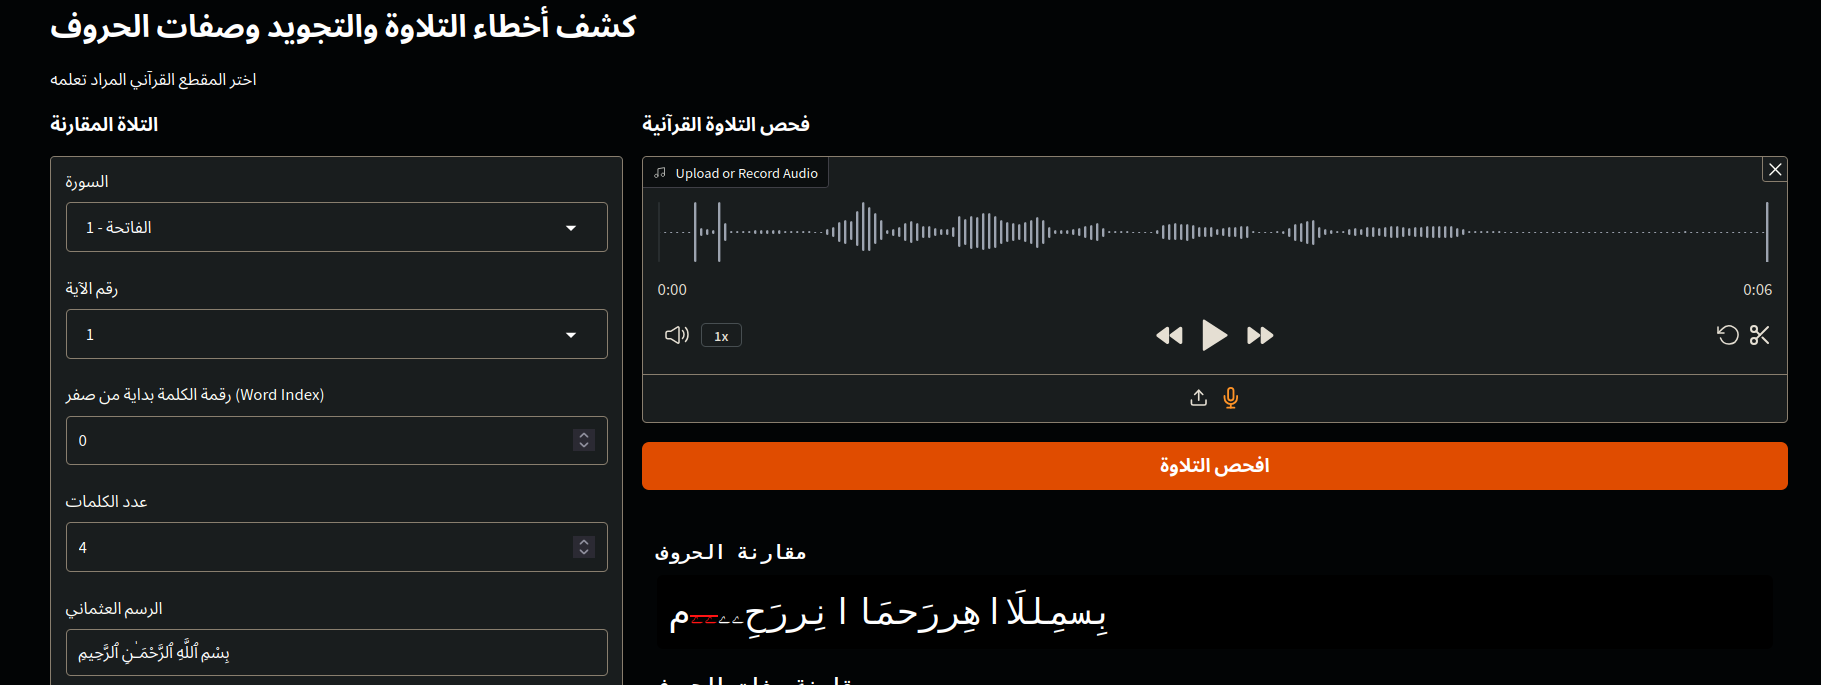
\includegraphics[width=0.8\textwidth]{../figures/gradio_ui_main.png}
\caption{Gradio Web App interface allowing users to test our model.}
\label{fig:gradio_main}
\end{figure}

\begin{figure}[H]
\centering
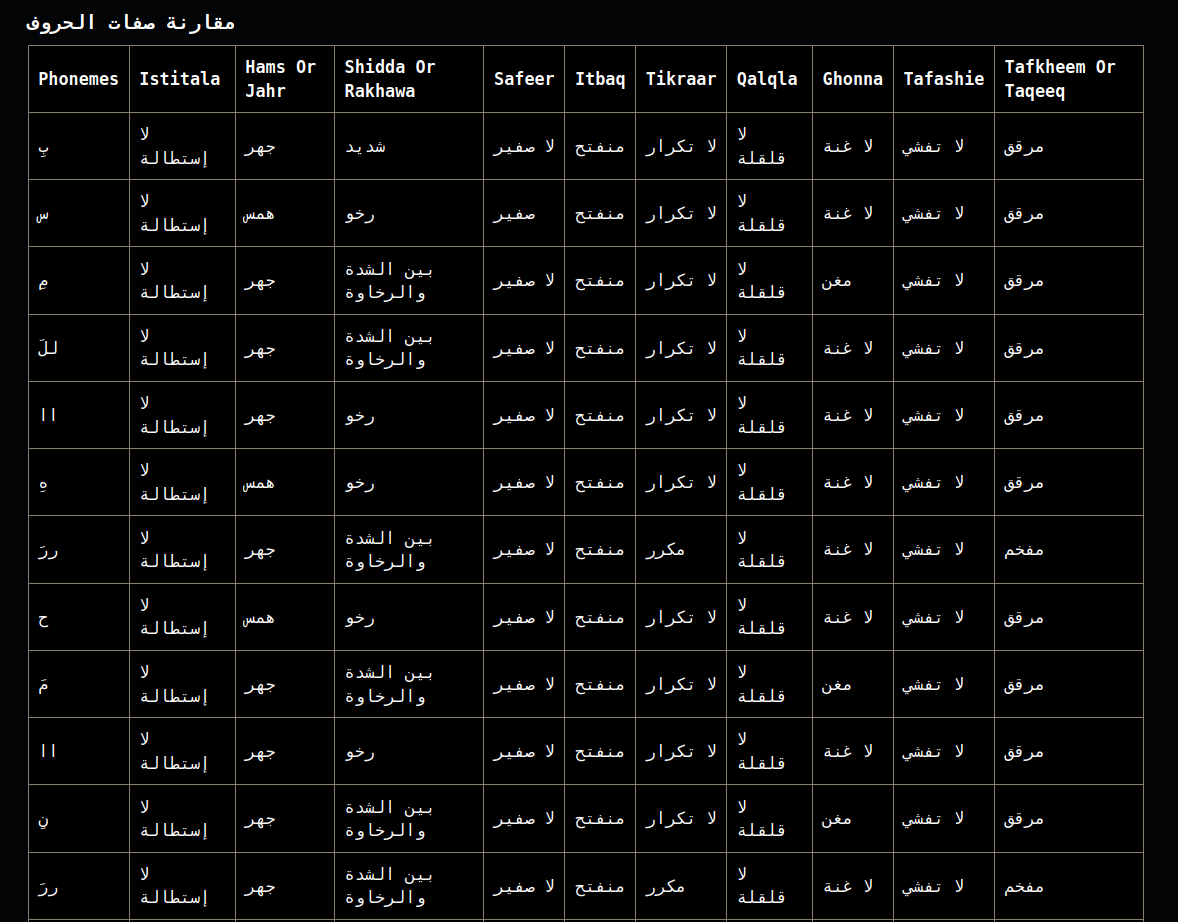
\includegraphics[width=0.8\textwidth]{../figures/gradio_ui_sifa.png}
\caption{Gradio Web App interface showing detailed Sifat (attribute) level feedback.}
\label{fig:gradio_sifa}
\end{figure}

User feedback has been extremely positive. Notably, the model generalized well to female voices despite being trained exclusively on male recitations, successfully detecting common errors such as incorrect \arb{مد} elongation or weak \arb{قلقلة} pronunciation. This demonstrates the robustness and practical applicability of our approach.
